\chapter{Podstawy teoretyczne}
\section{Wyznaczanie położenia na podstawie odległości od punktów stałych}

Zadaniem prezentowanego prototypu jest wyznaczenie położenia nadajnika na podstawie jego 
odległości od znanych punktów stałych. Niech $\boldsymbol{x}$ będzie szukanym punktem w przestrzeni,
$\boldsymbol{y_1,y_2,y_3}$ stałymi punktami o znanym położeniu, a $r_1,r_2,r_3$ wyznaczonymi odległościami
(rysunek \ref{fig:polozenie}).

\rysunekW{polozenie}{Wyznaczenie położenia na podstawie odległości od punktów stałych}{\label{fig:polozenie}}{0.7}
Wtedy $\boldsymbol{x}$ możemy wyznaczyć za pomocą układu równań:
 \begin{align}
    \nonumber |\boldsymbol{y_1} - \boldsymbol{x}| &= r_1,
 \\ \nonumber |\boldsymbol{y_2} - \boldsymbol{x}| &= r_2,
 \\ \nonumber |\boldsymbol{y_3} - \boldsymbol{x}| &= r_3,
 \end{align}
co dla przestrzeni euklidesowej daje:
 \begin{align}  
    \nonumber   (y_{11}-x_1)^2 + (y_{12}-x_2)^2 + (y_{13}-x_3)^2 &= r_1^2,
 \\ \nonumber   (y_{21}-x_1)^2 + (y_{22}-x_2)^2 + (y_{23}-x_3)^2 &= r_2^2,
 \\ \nonumber   (y_{31}-x_1)^2 + (y_{32}-x_2)^2 + (y_{33}-x_3)^2 &= r_3^2.
 \end{align}

Zauważmy, że znając odległość $\boldsymbol{x}$ od jednego z punktów stałych, wiemy, że $\boldsymbol{x}$ będzie leżał na
sferze o promieniu równym danej odległości. Znając dwie odległości, możemy ograniczyć poszukiwania do części wspólnej dwóch sfer,
czyli na ogół okręgu. Dla znanych trzech odległości dostajemy część wspólną okręgu ze sferą, czyli zwykle dwa możliwe punkty.
Mimo iż trzy odległości nie są wystarczające do jednoznacznego wyznaczenia $\boldsymbol{x}$, 
to otrzymane rozwiązania są na ogół od siebie odległe i 
możemy założyć, że jedno z rozwiązań jest szukanym przez nas punktem.

Ponieważ mamy pełną dowolność w doborze punktów stałych $\boldsymbol{y_i}$, dla uproszczenia możemy przyjąć:
$\boldsymbol{y_1}=(\frac{a}{2},0,0), \boldsymbol{y_2}=(-\frac{a}{2},0,0), \boldsymbol{y_3}=(0,h,0)$. 
Zatem $\boldsymbol{y_1}, \boldsymbol{y_2}, \boldsymbol{y_3}$ są wierzchołkami
trójkąta równoramiennego o wysokości $h$ i podstawie $a$, natomiast układ równań upraszcza
się do postaci:
 \begin{align}
    \nonumber  (\frac{a}{2}-x_1)^2 + x_2^2 + x_3^2 &= r_1^2,
 \\ \nonumber  (\frac{a}{2}+x_1)^2 + x_2^2 + x_3^2 &= r_2^2,
 \\ \nonumber  x_1^2 + (h-x_2)^2 + x_3^2 &= r_3^2,
 \end{align}
z czego ostatecznie otrzymujemy:
 \begin{align}
    \nonumber  x_1 &= \frac{r_2^2 - r_1^2}{2a},
 \\ \nonumber  x_2 &= \frac{r_2^2 - r_3^2 + x_1^2 - (\frac{a}{2}+x_1)^2}{2h}  + \frac{h}{2},
 \\ \nonumber  x_3 &= \pm \sqrt{r_3^2-x_1^2-(h-x_2)^2}.
 \end{align}


\section{Wyznaczanie orientacji w przestrzeni}

Oprócz położenia nadajnika w przestrzeni interesuje nas również jego orientacja.
Standardowo zdefiniuje się ją jako kąty Eulera \cite{bib:katyEulera}: przechylenia, 
pochylenia oraz odchylenia wokół osi związanych z obiektem, jednak na potrzeby niniejszej pracy wygodniej 
posługiwać się dwoma prostopadłymi wektorami, które jednoznacznie wyznaczają owe kąty. 
Prezentowany prototyp określa położenie czterech punktów $\boldsymbol{x_1, x_2, x_3, x_4}$ będących wierzchołkami prostokąta 
znajdującego się na nadajniku, a następnie na ich podstawie wyznacza poszukiwane dwa prostopadłe wektory, które jednoznacznie
definiują jego orientację (rysunek \ref{fig:orientacja}).
 \begin{figure}[H]
    \centering
    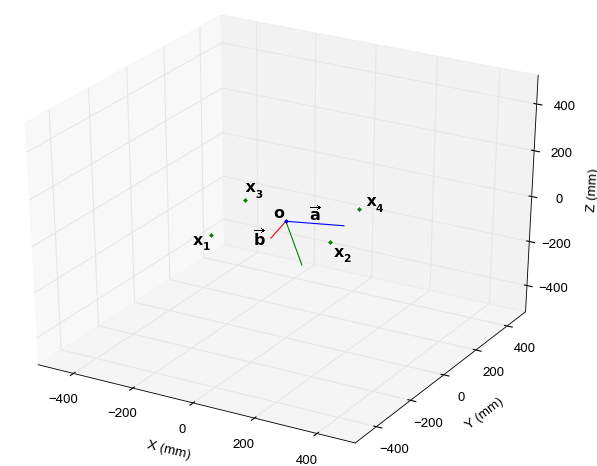
\includegraphics[width=0.5\textwidth, trim= 0mm 0mm 0mm 0mm,clip]{orientacja}
    \caption{Wyznaczanie orientacji na podstawie czterech punktów}
    \label{fig:orientacja}
\end{figure}
Na rysunku punkt $\boldsymbol{o} = (\boldsymbol{x_1} + \boldsymbol{x_2} + \boldsymbol{x_3} + \boldsymbol{x_4})/4$ jest szukanym położeniem
nadajnika, a~wektory $\boldsymbol{\overrightarrow{a}} = (\boldsymbol{x_2} + \boldsymbol{x_4})/2 - \boldsymbol{o}$ oraz 
$\boldsymbol{\overrightarrow{b}} = (\boldsymbol{x_1} + \boldsymbol{x_2})/2 - \boldsymbol{o}$ wyznaczają jednoznacznie
orientację przestrzenną nadajnika.

Zauważmy, że wyznaczenie położenia czterech punktów w przestrzeni daje nam pewną nadmiarowość
danych. Do wyznaczenia pozycji nadajnika potrzebujemy jedynie trzech współrzędnych,
a dla orientacji -- zaledwie trzech kątów, czyli w sumie sześciu niewiadomych.
Prezentowany prototyp wyznacza  dwanaście niewiadomych, co daje dwukrotną nadmiarowość danych.
Jest to efekt pożądany, gdyż pozwala na korektę błędów pomiarowych.


\section{Pomiar odległości za pomocą ultradźwięków}

Prezentowane urządzenie do pomiaru odległości wykorzystuje metodę pomiaru czasu, jakiego
potrzebuje dźwięk, aby pokonać drogę od nadajnika do odbiornika
(rysunek \ref{fig:pomiar_odleglosci}).
\rysunekW{pomiar_odleglosci}{Pomiar odległości za pomocą ultradźwięków}{\label{fig:pomiar_odleglosci}}{0.4}

Znając prędkość rozchodzenia się fal dźwiękowych w powietrzu oraz czas, jakiego fala dźwiękowa potrzebowała
do pokonania danego dystansu, jesteśmy w stanie wyznaczyć szukaną odległość.

Prędkość dźwięku w powietrzu w dużym stopniu zależy od panujących warunków atmosferycznych \cite{bib:soundSpeed},
zwłaszcza temperatury.
Dla gazu doskonałego prędkość ta wyraża się wzorem:
\[
V = \num{331,3}  \sqrt{1+\frac{T}{\num{273,15}}} \qquad \left[ \SI{}{\frac{m}{s}} \right]
\]

gdzie $T$ jest temperaturą w stopniach Celsjusza (\SI{}{\degC}).
Wzór ten możemy przybliżyć za pomocą rozwinięcia Taylora dla temperatur bliskich temperaturze pokojowej \ang{25}\SI{}{C}:
\[
 V = \num{346,13}  +  \num{0,580}(T - \ang{25})  \qquad \left[ \SI{}{ \frac{m}{s}} \right]
\]

Mimo że współczynnik temperaturowy jest stosunkowo mały i stanowi jedynie 0,17\% całej prędkości,
to przy odległościach rzędu metrów i rozdzielczościach rzędu milimetrów staje się on istotny, 
dlatego w przypadku prezentowanego prototypu niezbędna jest kalibracja wstępna, która pozwala
wyznaczyć aktualną prędkość dźwięku.





